\documentclass[journal]{new-aiaa}
%\documentclass[conf]{new-aiaa} for conference papers
\usepackage[utf8]{inputenc}

\usepackage{graphicx}
\usepackage{amsmath}
\usepackage[version=4]{mhchem}
\usepackage{siunitx}
\usepackage{longtable,tabularx}
\usepackage{gensymb}
\usepackage{caption}
\usepackage{subcaption}
\setlength\LTleft{0pt} 

\title{HabPi: An Open Source Extensible Framework for High Altitude
Balloon Data Collection}

\author{Robert Lowe\footnote{Assistant Professor, Division of
Mathematics and Computer Science, Maryville College, 502 East Lamar
Alexander Parkway, Maryville TN 37804}}
\affil{Maryville College}

\begin{document}

\maketitle

\begin{abstract}
One of the obstacles facing beginning high altitude balloonists
is the cost of the myriad sensors required to acquire usable data.
In addition to this problem, aligning sensor data after a flight can
prove tricky.  Finally, there is a harsh reality we all face.  Trees
exist, and payload stacks are attracted to trees!

HabPi is an open source project which attempts to address these
problems.  This is a sensor array which is based on a Aaspberry Pi,
a Sense HAT, and several one-wire sensors.  The sensors are all
synchronized, so data registration is not a problem.  HabPi also acts
as a wifi access point which makes data retrieval possible even when
the stack is trapped in a tree (or is otherwise inaccessible).  HabPi
is a simple extensible framework which allows users to add additional
experiments beyond the default setup.  The default setup provides
temperature, pressure, magnetometer, gyroscope, accelerometer, and
video imaging all for less than \$200.00.
\end{abstract}

\section{Introduction}
The HabPi project is both an open source software package and
a recommended hardware configuration.  The aim of this project is to
provide a simple and extensible high altitude sensing system which is
both economical and robust. The default configuration of the HabPi
system results in a platform capable of capturing the following data:
\begin{itemize}
    \item Temperature
    \item Humidity
    \item Barometric Pressure
    \item Magnetometer Data
    \item 3-Axis Accelerometer Data
    \item 3-Axis Gyroscope Data
    \item Still Photos / Video
\end{itemize}
In addition to these basic data points, the system provides many
opportunities for expansion.  For example, there have been flights
carrying cosmic ray detection experiments using a similar hardware
setup.  

In addition to its low cost, this system provides a central point of
contact for all sensor data.  This means synchronization of recorded
data is trivial as all data points are recorded with a common
clock.  In fact, data recording procedures can be crafted which
concurrently capture data points the user is interested in comparing,
thus eliminating the challenges of synchronizing data across disparate
sensors.

A final advantage present in the current system is in the recovery of
data.  If the payload can be recovered, then the on board computer is
sufficient to process the information obtained during the flight.  If
the payload is not recoverable, the HabPi system provides a mechanism
for wireless transmission of the data.  Thus, so long as a user can
get to within a few hundred feet of the payload, the data will always be
recoverable and usable. (Provided, of course, the payload lands
intact.)

\subsection{Motivation}
The primary motivation for the creation of the HabPi system was cost.
When presented with the prospect of beginning a ballooning program, it
is easy to become overwhelmed with the choices of available sensors
and the costs of their given platforms.  Also, many of these platforms
necessitate the use of proprietary software.  This can create
a situation where experimental efforts are stymied by the lack of
control inherent in these sorts of systems.

Another motivation for the creation of HabPi in its present form was
the loss of a payload in November of 2016.  The first HabPi payload launched
by a joint effort between Maryville College and Pellissippi State
Community College came to rest at the top of a very large tree in
Pisgah National Forest.  While the payload was sited, and indeed
visited on five occasions, all of the precious data from the flight
was trapped some 65 feet above the ground.  The addition of wireless
download capabilities was a natural result of the frustration from
this all to common event.

\subsection{Educational Use}
In addition to its use in normal stratospheric flight experiments,
HabPi has also proved to be very useful in education.  It was
developed and refined using input from students at Maryville College
and Pellissippi State Community College.  In addition to college
students, HabPi payloads have also been constructed by elementary,
middle, and high school students from Concord Christian School.  Boy
Scout Troop 255 also built and flew a HabPi payload. As can be
expected, the students were all very excited to participate in
a stratospheric flight.

In addition to collecting stratospheric data, the default setup of
a HabPi system works well as a ground based weather station.
Curricula including weather experiments culminating in a stratospheric
flight are currently under development, and will hopefully be the topic
of a future paper.

\subsection{Organization of this Paper}
The remainder of this paper is organized as follows.  First, the
construction of the HabPi payload is outlined.  This includes both the
sensor hardware and the recommended box dimensions.  Following the
construction section is a detailed description of the HabPi software,
including both setup and operation.  The final two sections of the
paper present flight data and some concluding remarks about the
performance of the HabPi system. 

\section{Construction}
The HabPi setup consists of four principal components:
\begin{enumerate}
    \item A Raspberry Pi version 3 Computer~\cite{RaspberryPi}
    \item A Sense HAT board~\cite{SenseHat}
    \item Raspberry Pi Camera V2~\cite{RaspberryPi}
    \item Three DS18B20 1-Wire Temperature Sensors~\cite{DS18B20}
\end{enumerate}
A complete parts list for the electronics, along with approximate
cost, can be found in Table~\ref{tab:parts}.

The Raspberry Pi computer is designed to be a friendly Linux based
system which is easily programmable.  Of particular interest is the
presence of both USB ports and an array of programmable GPIO (General
Purpose IO) pins.  This allows the Raspberry Pi to serve as both
a driver and processor for sensors using a variety of communication
technologies.  In addition to its wired connections, the Raspberry Pi
version 3 also provides wireless connectivity in the form of bluetooth
and wifi.  This later adapter can be configured to act as a wifi
access point, allowing the Raspberry Pi to function as the hub of
a wireless network.

\begin{table}
    \begin{center}
    \begin{tabular}{l|r}
        {\bf Item} & {\bf Approximate Cost}\\
        \hline
        Raspberry PI 3 Model B. & \$35.00\\
        Sense HAT & \$30.00\\
        Raspberry Pi Camera V2& \$30.00\\
        32GB Micro SD Card & \$15.00\\
        3 $\times$ DS18B20 Digital Thermometers & \$9.00\\
        4.7k$\Omega$ 1/4 W Resistor & \$0.10\\
        30 Row self-adhesive breadboard & \$5.00\\
        4400 mAh USB Battery (Cell Phone Charger) & \$10.00\\ 
        20 pack of Male/Female Jumper Wires & \$3.00\\
        300mm Ribbon Cable for Pi Camera & \$2.00\\
        \hline
        {\bf Total} & {\bf\$139.10} \\
    \end{tabular}
    \caption{Parts List}
    \label{tab:parts}
    \end{center}
\end{table}

The Sense HAT board is an array of sensors which was designed to be
part of the Astro Pi mission~\cite{MagpiSenseHat}.  
A device containing both a Raspberry Pi and a Sense HAT was sent to
the international space station.  Children from around the world
contributed experiments as part of a contest where the winners had
their experiments carried out aboard the ISS.  The Sense HAT provides
the following features:
\begin{itemize}
    \item Two Digital Thermometers ($-40 \celsius$ to $+120 \celsius$)
    \cite{HTS221} and ($-30 \celsius$ to $+105 \celsius$)\cite{LPS25H}
    \item Barometric Pressure Sensor (260 to 1260 hPa) ~\cite{LPS25H}
    \item Relative Humidity Sensor ($0\%$ to $100\%$)~\cite{HTS221}
    \item 3-Axis Magnetometer ($\pm 16$ gauss)~\cite{LSM9DS1}
    \item 3-Axis Gyroscope ($\pm 2000$ dps)~\cite{LSM9DS1}
    \item 3-Axis Accelerometer ($\pm 16$g)~\cite{LSM9DS1}
    \item Joystick for Input
    \item RGB LED Array for Output
\end{itemize}

Of course, the temperature ranges provided by the Sense HAT are not
sufficient for recording stratospheric temperatures.  Moreover,
because the Sense HAT itself becomes warm during normal operations, the
temperatures read by the Sense HAT will tend to be higher than the
ambient temperature~\cite{SenseHat-API}.  To combat this, the standard
HabPI setup uses 3 DS18B20 1-wire thermometers which have an
advertised temperature range of $-55\celsius$ to
$+125\celsius$~\cite{DS18B20}.

\subsection{Wiring the Sense HAT}
\begin{figure}
    \centering
    \begin{subfigure}{.45\textwidth}
        \centering
        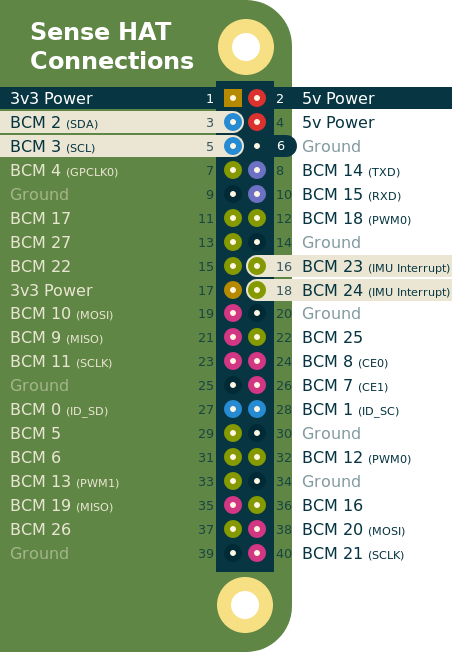
\includegraphics[width=2.75in]{images/rpi-sensehat}
        \caption{Minimal Raspberry Pi Sense HAT
        Connections~\cite{pinout}}
        \label{fig:pinout}
    \end{subfigure}
    \begin{subfigure}{.45\textwidth}
        \centering
        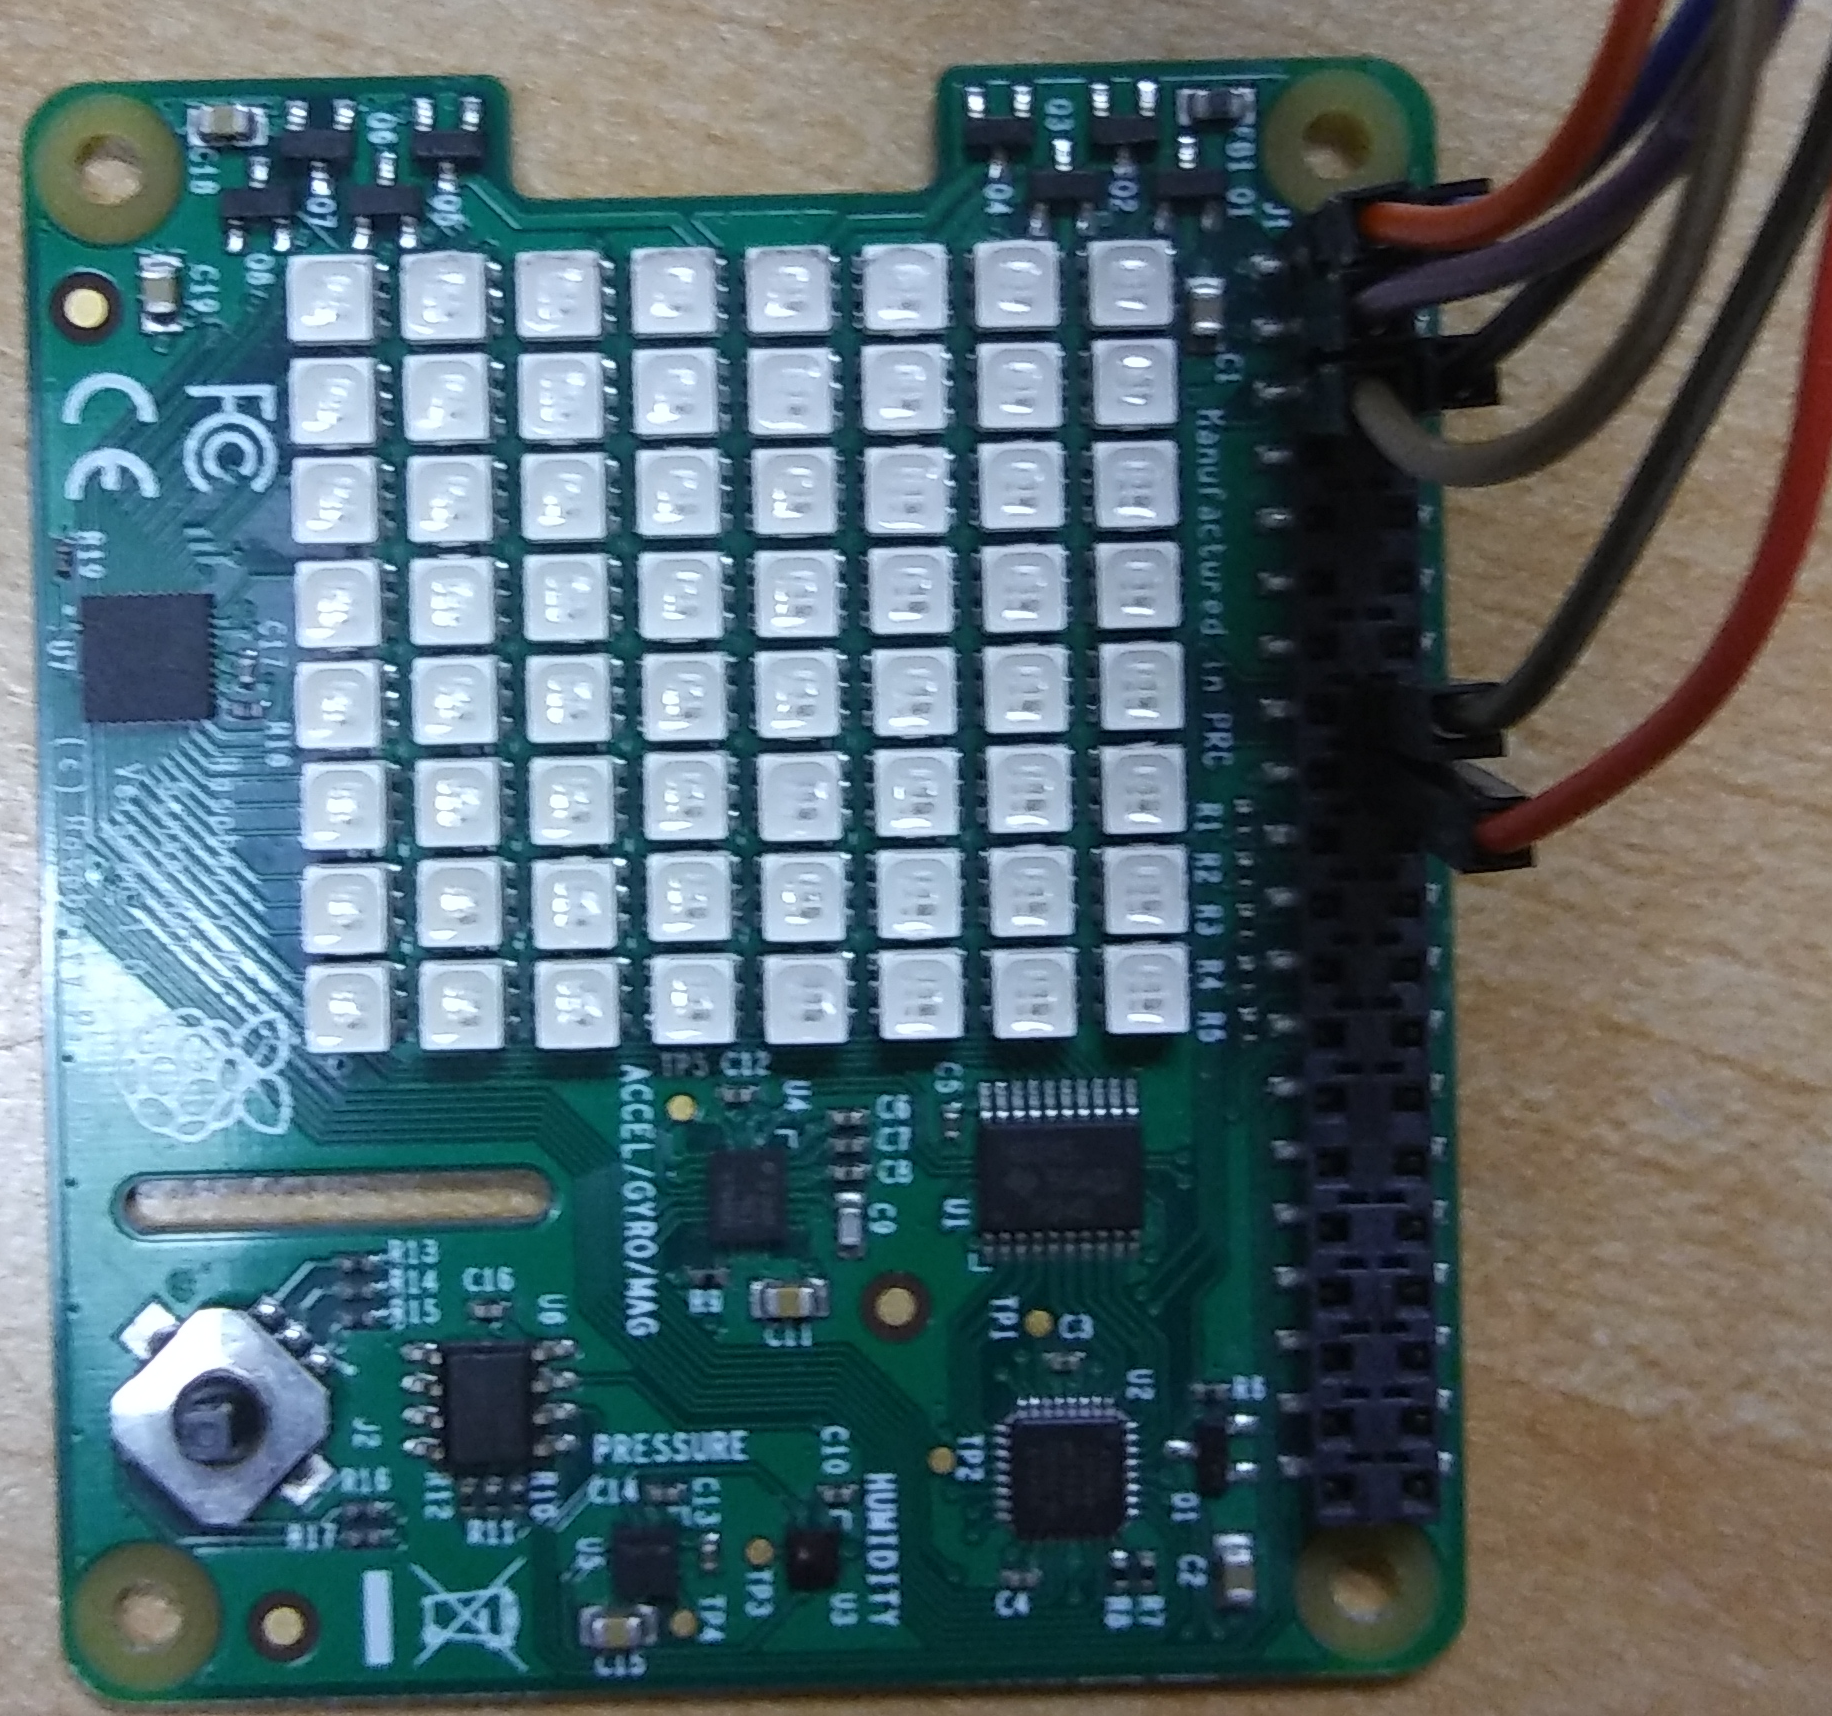
\includegraphics[width=2.75in]{images/sensehat}
        \caption{Sense Hat Connections}
        \label{fig:hat}
    \end{subfigure}
    \caption{Wiring the Sense Hat}
    \label{fig:hatwiring}
\end{figure}

Out of the box, the Sense HAT has a connector which fits over all of
the Raspberry Pi's GPIO pins.  This is undesirable for two reasons.
First, this means no further GPIO hardware can be added.  Second, and
most importantly, the heat from the Raspberry Pi will dramatically
increase the temperature read by the Sense HAT.  Fortunately, this
connector can be removed by simply pulling it out of the Sense HAT.
To wire the Sense HAT, only seven connections are actually necessary.
These connections are shown
in Figure \ref{fig:pinout}, with figure \ref{fig:hatwiring} showing
the corresponding orientation of the Sense HAT.  These connections are
made using Male/Female jumper wires.

\subsection{Wiring the 1-Wire Sensor Array}
\begin{figure}
    \centering
    
\includegraphics[height=3.5in]{images/ds18b20-circuit}
    \caption{DS18B20 1-Wire Circuit}
    \label{fig:circuit}
\end{figure}
The DS18B20 1-wire sensors share a common data line which is connected
to a pull-up resistor.  It should be noted that any number of 1-wire
sensors can share this single pull-up resistor.  The power and ground
of each of the sensors is connected to the 3v3 and GND line on the Raspberry
Pi respectively.
This circuit is built on a solderless breadboard using the jumper
wires according to the schematic shown in Figure~\ref{fig:circuit}. 

\subsection{Box Dimensions and Mounting}
\begin{figure}
    \centering
    \begin{subfigure}{0.45\textwidth}
        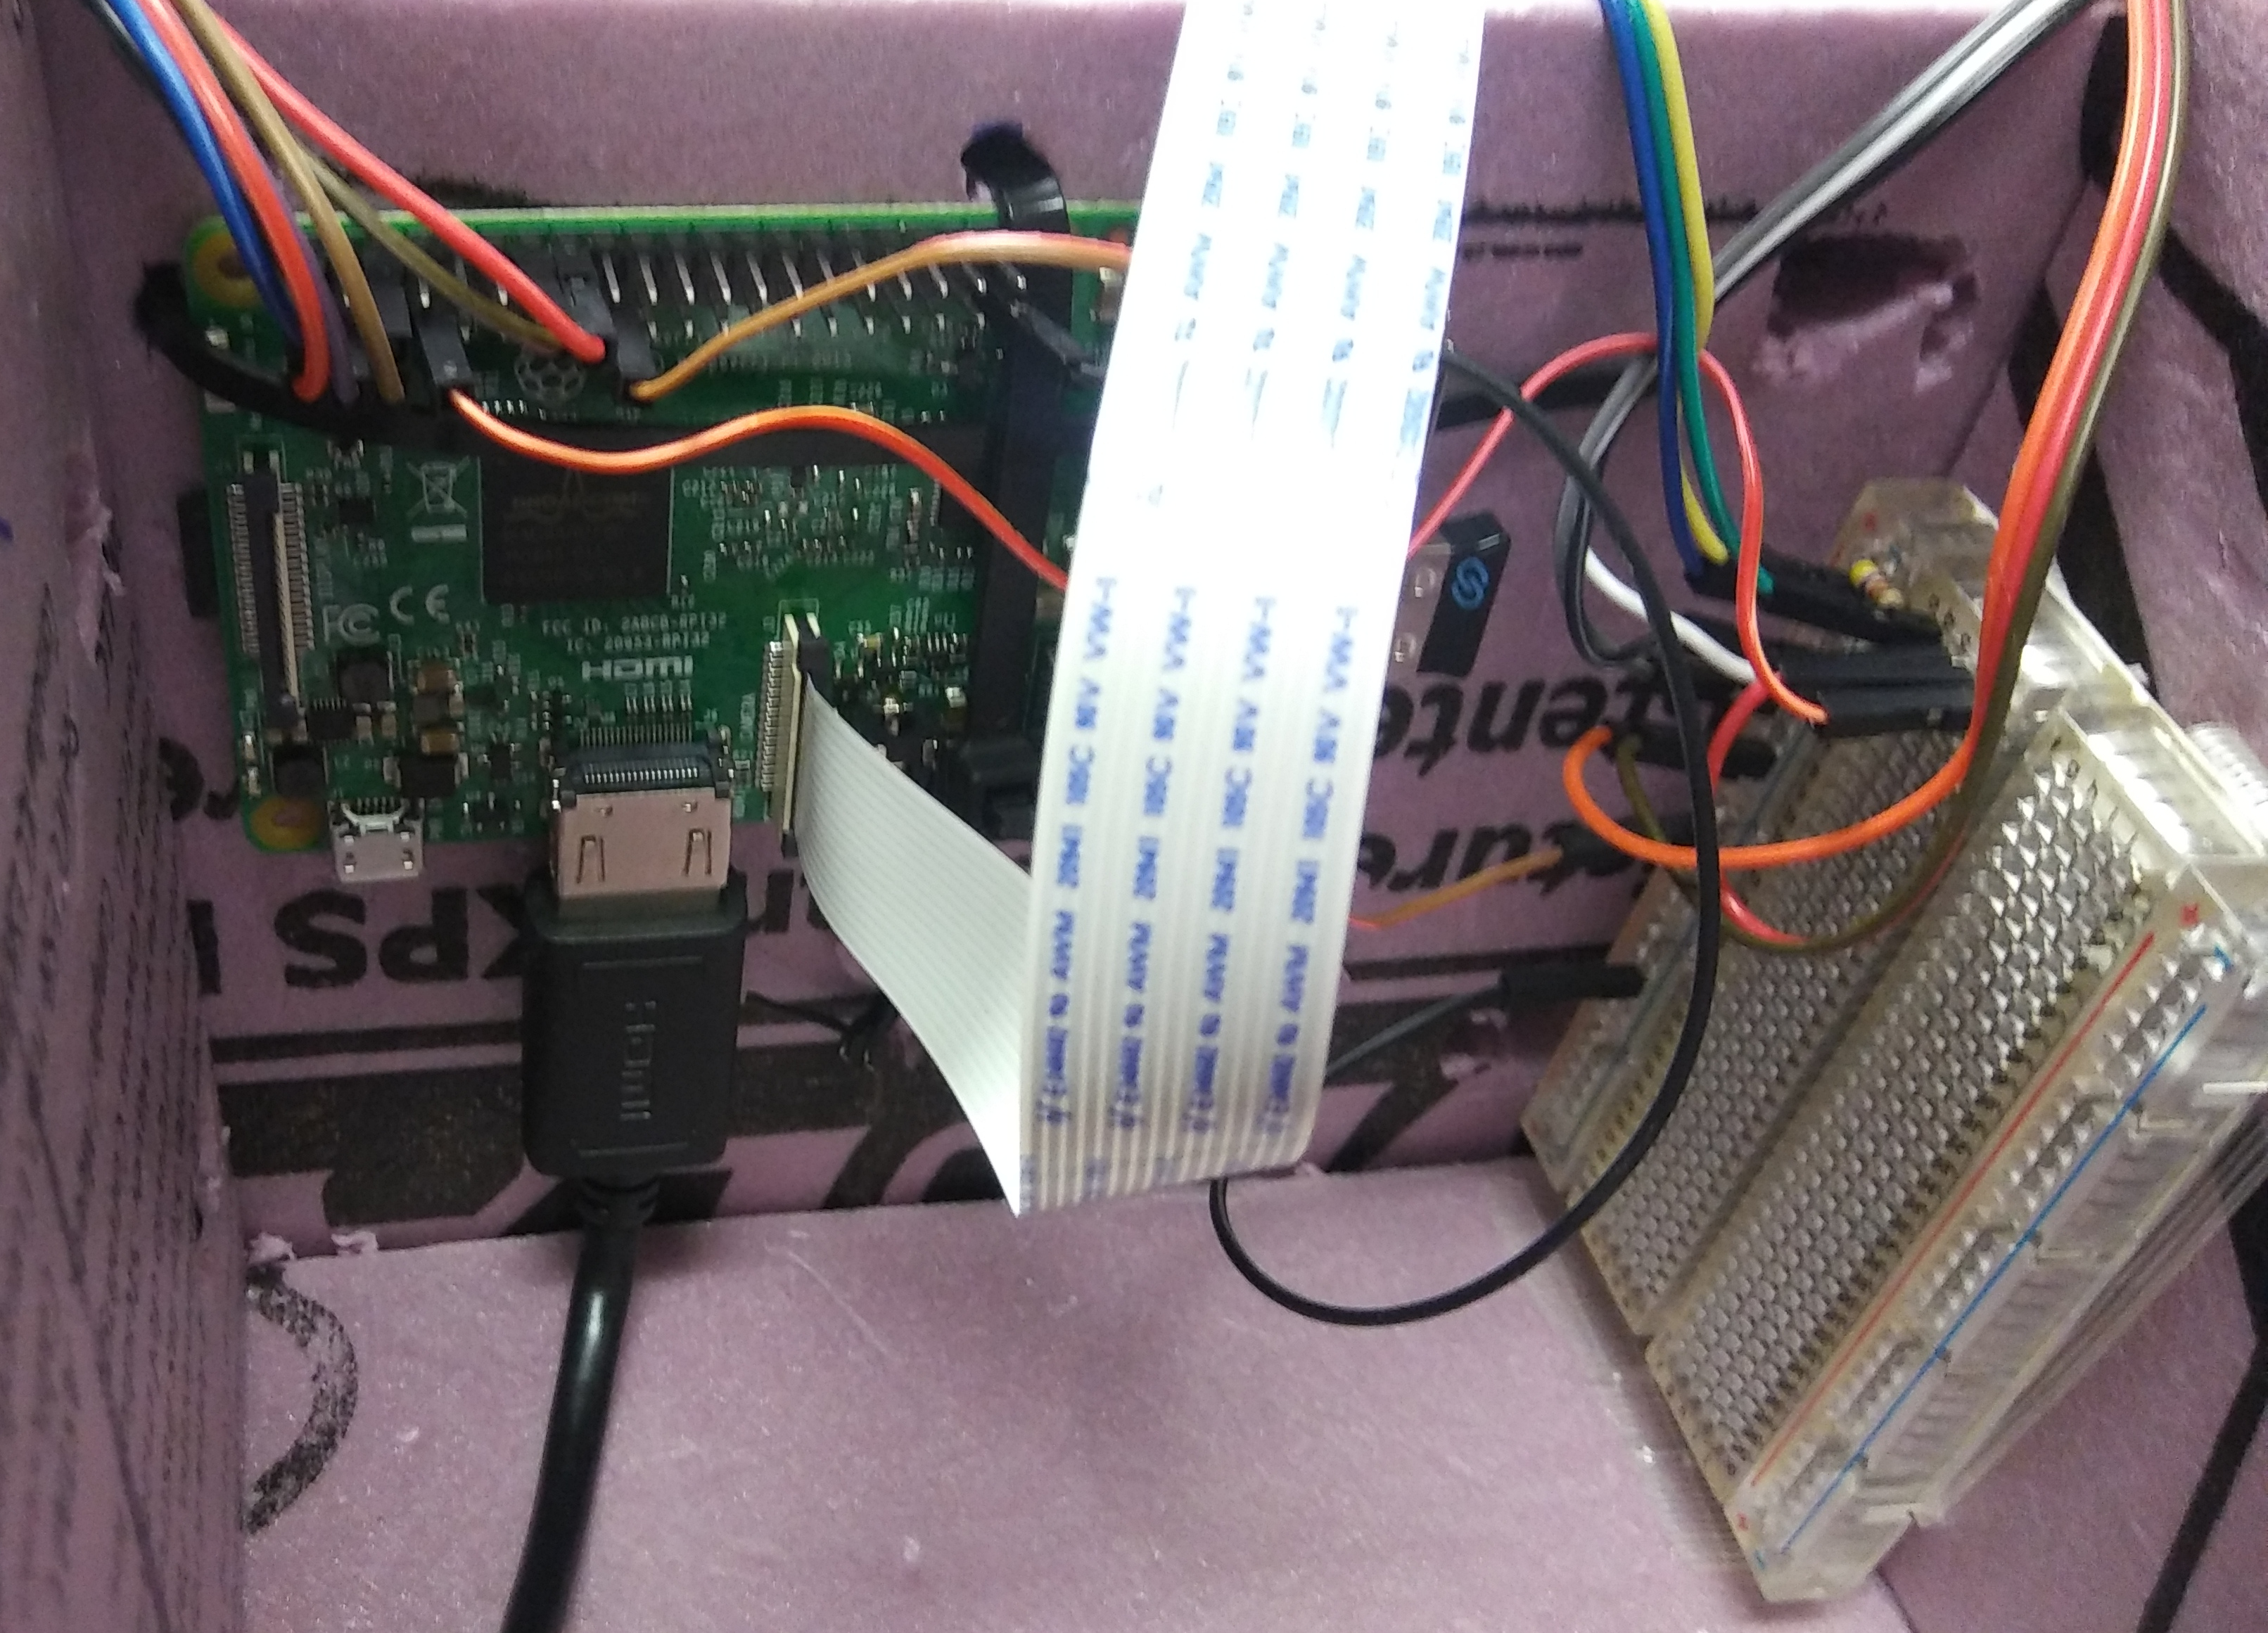
\includegraphics[width=2.75in]{images/interior}
        \caption{Interior with Mounted Computer and Breadboard}
        \label{fig:interior}
    \end{subfigure}
    \begin{subfigure}{0.45\textwidth}
        \includegraphics[width=2.75in]{images/top}
        \caption{Top Showing Mount Points for the Sense HAT}
        \label{fig:top}
    \end{subfigure}
    \caption{Mounting the Electronics}
\end{figure}
The recommended payload enclosure for HabPi has exterior dimensions of
$8"\times8"\times8"$ and interior dimensions of $6"\times6"\times6"$.
This provides ample room to mount the base setup and still access the
display and power ports of the Raspberry Pi.  This also provides
enough room to add additional experiments to the box.  Of course, the
enclosure can be any dimensions the user wishes, so long as the wires
can be made to reach.  The self adhesive breadboard is affixed to the
inside of the box, and the battery is mounted to the bottom.  The
suggested layout of the inside of the box is shown in
Figure~\ref{fig:interior}.

In order to isolate the Sense HAT from the heat generated by the other
components, it is mounted to the lid of the box on the outside.  The
easiest way to mount the Sense HAT is by passing wire through the foam
at the corners and twisting it on the other side of the lid.
Figure~\ref{fig:top} shows the positioning of the Sense HAT along with
markings for the wire mount holes.

The camera is mounted in the same fashion on the outside of the box.
This can be positioned wherever the user desires.  Also, tape should be
applied to the ribbon cable to secure it to the outside of the box.
One advantage of using the Raspberry Pi camera in this fashion is that
it does not require large holes to be cut into the insulation of the
payload box.

The temperature sensors are all connected to jumper wires and left to
dangle freely.  The suggested way to fly these sensors is with two on
the outside of the box and one on the inside of the box in order to
measure the efficacy of the insulation\footnote{This can be
a source of friendly competition when working with groups of
grade-school students! The winner is the group who's box stays warmer.}.

\section{HabPi Software}
The HabPi software is a series of python scripts which form
a framework for collecting data from the sensors.  The software is
released under the GPL3 license, and is available at TBD\footnote{I am
still working out hosting details.  This will be resolved within
a week or so. The final paper will include a URL to the software.}.

HabPi is designed to run on top of Raspbian Stretch, though it can be
used with other distributions on the Raspberry Pi. HabPi creates
a hierarchy of folders in the home directory of the pi user.  These
are as follows:
\begin{description}
    \item[habpi/] The HabPi distribution itself.
    \begin{description}
        \item[HabPi/] The HabPi python module.
        \item[data/] The collected data from HabPi.
        \item[scripts/] Utility scripts for the HabPi system.
        \item[experiments/] The experiment scripts to be executed when
        HabPi collects data.
        \item[examples/] Example Experiment Scripts
        \begin{description}
            \item[flash.py] A script which causes the LEDs
            on the Sense HAT 3 hours after activation.  (Useful for
            Recovery)
            \item[senseRec.py] A small script to capture all of the
            data from the Sense HAT in a format that can be played
            back using the Sense HAT emulator.
            \item[timeLapse.py] A time lapse photography script.  This
            captures one image per second.  The delay can be adjusted
            by changing the code.
            \item[video.py] A video recording script.  It captures 10
            minutes of video per file and then rotates to another
            file.  This is to decrease the chance of losing video data
            during power failure.
            \item[temp.py] A script which logs temperatures from all
            five thermometers into a CSV file.  It produces one
            reading per second.
        \end{description}
    \end{description}
\end{description}

Whenever HabPi records data, it creates a new directory under the
data folder named {\em date}-{\em Unix timestamp}.  Thus any number of
recordings can be stored, space allowing.

\subsection{Raspberry Pi Setup}
The first step in setting up HabPi is to prepare the Raspberry Pi.
To do this, install Raspbian and then set up the localization options.
Change the default password, and then activate both the camera and ssh
interfaces.  Finally, install {\em hostapd} and {\em dnsmasq}.  These
last two are needed to allow the Raspberry Pi to act as a wifi access
point.

To complete the setup, we add the following line to the crontab of the
raspberry pi user:
\begin{verbatim}
@reboot /home/pi/habpi/scripts/start
\end{verbatim}

\subsection{Setting up HabPi}
The primary configuration for HabPi is located in the file {\tt
HabPi/config.py}.  The default configuration is to have HabPi act as
an access point with the SSID of ``SkyNet'' and the password of
``Terminat0r''. This can be changed, however.  When running as an
access point, no wifi internet connection is possible, but the Raspberry
Pi can still be connected to the internet via wired ethernet.
Setting the {\tt accessPoint} variable to {\tt False} will cause the
system to use client mode wifi instead.  

\subsection{Creating Experiments}
The final step in preparing to fly is to create the experiments.  Any
file ending in {\tt.py} contained in the experiments folder will be
executed in its own thread when data recording begins.  What these
experiments do is completely free form, but a good first step would be to
copy examples into the experiments folder.  It should be noted that
the video and time lapse examples are mutually exclusive.  The system
cannot do both at once due to the limitations of the Raspberry Pi
camera API.

Experiments should import the "HabPi" module.
This module provides the following information:
\begin{description}
    \item[HabPi.sense] The Sense HAT object.  This should be used
    instead of a manual connection so that the experiment can use the
    emulated Sense HAT if it is configured.
    \item[HabPi.dir] The full path to the data directory.  The
    experiment should record data here.
    \item[HabPi.sensors] Sensor states.  This is a dictionary which
    each experiment can publish information.  This allows inter-script
    communication.
\end{description}

Once the experiments are in place, HabPi is ready to run.

\subsection{HabPi User Interface}
When the system reboots, HabPi will automatically start.  The LEDs
will begin flashing a question mark ``?'', as a prompt.  There are
then two ways to interact with HabPi. 

\subsubsection{Sense HAT Joystick}
Pressing up on the joystick will cause HabPi to enter ``Date Set''
mode.  This will allow the date to be set using the joystick one digit
at a time.  Pressing right on the joystick allows the user to enter
the current time.  Pressing left on the joystick will display the
current date and time.  These are necessary because the Raspberry Pi
lacks a real time clock.  (Adding one is a fun project, but by default
there is not one present.)  Thus it needs to have its time reset every
reboot. Pressing down on the joystick will cause HabPi to count down.
It will display the sequence 3, 2, 1.  Pressing the joystick during
the count down will cancel the recording and return to the prompt.
Otherwise HabPi will flash an ``R'' to indicate that it has started
recording data.

\subsubsection{Built-In webserver}
Another option for controlling HabPi is via its built-in webserver.
Using a mobile device, join HabPi's network.  From there visit {\tt
http://172.24.1.1:8080} which provides the user with an interface
which can set HabPi's time, start
the experiments, stop the experiments, and download data.

\section{Performance and Flight Data}
The data in this section are from a stratospheric flight which took
place on October 7, 2017.  The balloon was released from Athens, TN 
at approximately 14:00 UTC and the payload was recovered in 
Knoxville, TN four hours later.  The balloon reached a peak altitude
of 82,789 feet according to the Iridium satellite tracker which was
part of the payload stack.

\subsection{Temperature Data}
\begin{figure}
    \centering
    \begin{subfigure}{0.45\textwidth}
        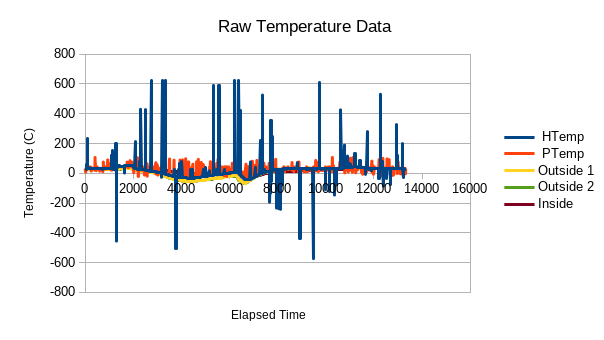
\includegraphics[width=2.75in]{images/rawtemp}
        \caption{Raw Temperature Data of All Sensors}
        \label{fig:rawtemp}
    \end{subfigure}
    \begin{subfigure}{0.45\textwidth}
        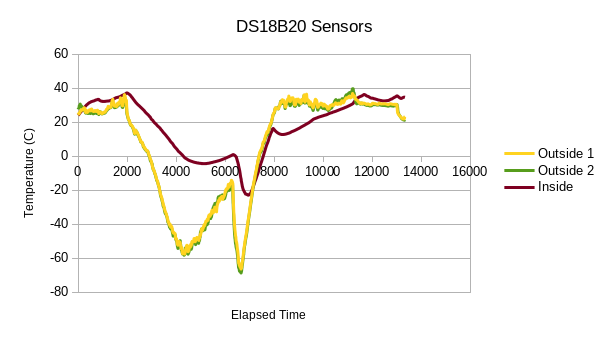
\includegraphics[width=2.75in]{images/ds18b20-data}
        \caption{ds18b20-data}
        \label{fig:ds18b20-temp}
    \end{subfigure}
    \begin{subfigure}{0.45\textwidth}
        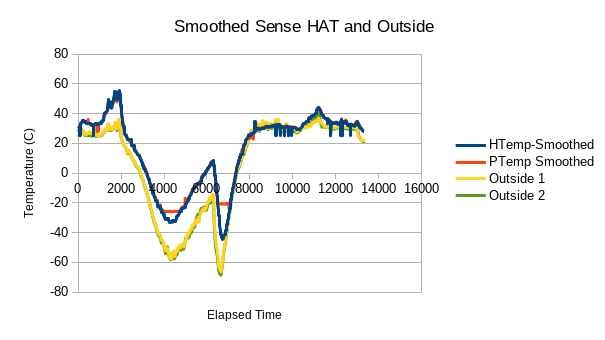
\includegraphics[width=2.75in]{images/smoothtemp}
        \caption{External Temperature data with Smoothed Sense HAT data}
        \label{fig:smooth}
    \end{subfigure}
    \caption{Temperature Data}
\end{figure}

The temperature data from this flight shows one of the key challenges
to using Sense HAT data.  The Sense HAT readings tend to be very
noisy, as can be seen in Figure~\ref{fig:rawtemp}.  The DS18B20
sensors, on the other hand, produce very clean information, as can be
seen in Figure~\ref{fig:ds18b20-data}.  Fortunately, smoothing the
Sense HAT data is fairly simple.  The filter applied in
Figure~\ref{fig:smooth} is accomplished by simply excluding any data
point which differs by more that $5\celsius$ from the previous data
point.  

As is predicted by the documentation of the Sense HAT, these
temperatures are warmer than the temperatures captured by the DS18B20
sensors.  Also, note that the DS18B20 sensors were painted white to
reduce solar heating.  The Sense HAT sensors cannot be painted as this
will interfere with their pressure and humidity readings.

\subsection{Other Sensors}
The other sensors in the Sense Hat are not quite as noisy as the
temperature sensors.  The pressure sensor has occasional spikes, but
in general it tracks well for the duration of the flight.  In this
flight, the pressure altitude reached by the balloon at its peak was
computed to be 85,388 feet.  

\begin{figure}
    \centering
    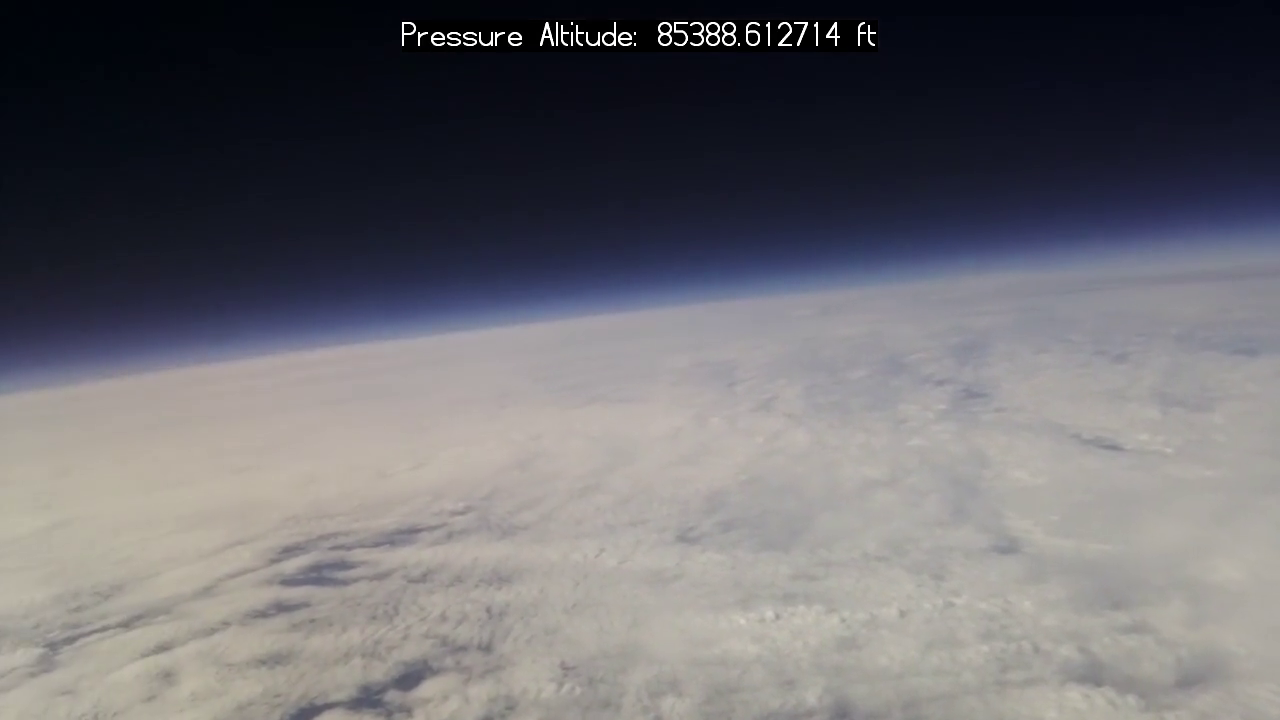
\includegraphics[width=0.75\linewidth]{images/peak-altitude}
    \caption{Peak Altitude with Overlay}
    \label{fig:peak}
\end{figure}

\section{Conclusion}
The HabPi system provides an open framework for high altitude sensing
based on readily available components.  It is simple to build, so much
so that it can be assembled by children, but it is also robust enough
to produce usable data.  Because the software is completely open
source, the user can alter all of the data collection routines to
suit their needs.  For example, one such extension is to overlay the
current pressure altitude on the captured video files, as seen in
Figure~\ref{fig:peak}.  The Raspberry Pi itself offers additional
1-wire capabilities as well as many available GPIO pins and USB ports.  

Future work will include the development of curricula for using HabPi
in classrooms, as well as more experiments driven by this framework.

\section{Acknowledgments}
The author would like to acknowledge Sarah Graham and the students of
Pellissippi State Community College for providing multiple
opportunities to build and fly HabPi payloads.  Special thanks to the
children of Concord Christian School and Troop 255 for building early
versions of HabPi payloads are also in order.

\bibliography{citations}
\end{document}
